\documentclass[a4paper,10pt]{report}
\usepackage[utf8]{inputenc}
\usepackage[italian]{babel}
\usepackage{graphicx}

% Title Page
\title{Visione GameShop+}
\author{Lorenzo Di Giuseppe, Matteo Gentile, Andrea Salini}

\begin{document}
  \maketitle

  
  \section*{Storico Revisioni}
  \begin{center}
    \begin{tabular}{|p{.13\textwidth} p{.13\textwidth} p{.4\textwidth} p{.22\textwidth}|}
      \hline
      \textbf{Versione} & \textbf{Data} & \textbf{Descrizione} & \textbf{Autore}\\
      \hline
      Bozza ideazione & 18.10.2013 & Prima bozza da raffinare
      successivamente & Matteo Gentile, Andrea Salini, Lorenzo Di Giuseppe\\
      \hline
    \end{tabular}
  \end{center}

  
  \section*{Introduzione}
  Prevediamo la realizzazione di un'applicazione di tipo POS, specifica per un negozio di
videogames. Il sistema è centrato sulla vendita di videogiochi, console, manuali,
accessori, gadget e sul loro scambio, prevedendo politiche di riciclo/rivendita dell'usato. Il
sistema deve prevedere flessibilità secondo regole di business diversificate (e.g. sconti,
scambi cliente-negozio...); inoltre si prevedono diversi punti d'accesso al sistema, quali i
terminali dei commessi del negozio e dei manager, e altri utilizzabili dai clienti, che in tal
modo possono svolgere ricerche sui prodotti, e altre operazioni in maniera autonoma.
Infine si prevede il supporto verso sistemi esterni prodotti da terze parti.

  \section*{Posizionamento}
  
  \subsection*{Opportunità di business}
  L'attuale sistema esistente nei negozi delle maggiori catene di vendita di videogiochi non
permette di consultare liste di prodotti, usati o nuovi, se non attraverso consultazione
manuale. Gli attuali sistemi quindi non consentono al cliente di informarsi sui prodotti a cui
è interessato, se non attraverso l'interazione con un commesso. Questo aumenta
sicuramente i tempi di attesa.
Il nostro obiettivo è quello di attaccare il mercato, offrendo un sistema robusto, flessibile ed
efficiente, che integri funzionalità di ricerca relativamente ad un punto di vendita,
mantenendo inalterate quelle che sono le attuali funzioni. I vantaggi in termini di tempo
risparmiato sarebbero notevoli; sia dal punto di vista degli impiegati del negozio che dei
clienti, con un conseguente aumento della soddisfazione generale.
Inoltre, supponendo che si tratti di una catena, il sistema, pur essendo mirato alla gestione
di un singolo punto di vendita, deve integrarsi con quelli di più alto livello, offrendo
funzionalità specifiche per un unico negozio.

  \subsection*{Formulazione del problema}
  I sistemi attuali prevedono la ricerca degli articoli tra gli scaffali. In caso di problemi un
cliente può chiedere aiuto al commesso, che può fornire indicazioni su dove trovare il
prodotto, ferma restando la possibilità che non sia presente in negozio.
In sostanza, non esiste un sistema informatico che consente la rapida consultazione della
merce, sia nuova che usata, disponibile presso un punto di vendita. Ovvero non è
possibile conoscere se ciò che si sta cercando sia disponibile fino a che non è stata svolta
una accurata ricerca manuale tra gli scaffali.

  \subsection*{Formulazione della posizione del prodotto}
  Il sistema è destinato a migliorare il rendimento dei centri di videogiochi, proponendosi
come alternativa agli attuali sistemi dei singoli negozi, offrendo integrazione con il sistema
della catena.

  \subsection*{Alternative e concorrenza}
  Sistemi attuali presenti nei negozi di videogiochi.
  
  \section*{Descrizione delle parti interessate}
  
  \subsection*{Riepilogo delle parti interessate (non utenti)...}
  Da considerare con particolare attenzione i fornitori, che sebbene non interagiscono
direttamente con il sistema, rappresentano una delle parti interessate al sistema.
  
  \subsection*{Riepilogo dell'utente....}
  Il sistema è rivolto ai commessi, manager e clienti del negozio, tutti direttamente in
contatto con esso.
  
  \subsection*{Obiettivi e problemi fondamentali ad alto livello delle parti interessate}
  \begin{tabular}{|p{.15\textwidth} p{.15\textwidth} p{.4\textwidth} p{.3\textwidth}|}
      \hline
      \textbf{Obiettivo di alto livello} & \textbf{Priorit\`a} & \textbf{Problemi} & \textbf{Soluzioni attuali}\\
      \hline
      Robustezza e
velocità del
completo
processo di
ricerca e vendita
del prodotto & 
Alta &  
Mancanza di
tecnologie a
supporto
dell'utente durante
la fase di ricerca
del prodotto.

Mancanza di
flessibilità nelle
tipologie di
acquisto.

Tempi lunghi per
l'acquisto, sia in
negozio (possibili
code o problemi di
ricerca) che da
casa (tempi di
spedizione
& 
Ricerca manuale
degli articoli.
Aiuto da parte del
commesso.
Acquisto online
con spedizione.\\
      \hline
Gestione fornitori &
Alta &
Presenza di
molteplici flussi in
ingresso; i clienti
sono fornitori di
prodotti usati.

I prodotti usati
sono oggetto di
politiche di
business. &
Da scoprire \\
\hline


      \end{tabular}
  
  \subsection*{Obiettivi a livello dell'utente}
  Gli utenti necessitano di un sistema che soddisfano i seguenti obiettivi.
  \begin{itemize}
   \item Commesso: Elaborare vendite, gestione resi, gestione scambi, cash in, cash out.
   \item Manager del negozio: Gestire magazzino, avviare il sistema, fermare il sistema.
   \item Amministratore: Inserire nuove politiche di business.
   \item Cliente: Ricercare e acquistare i videogiochi.
  \end{itemize}

  \subsection*{Ambiente dell'utente...}
  L’Utente si rega in un Game Shop principalmente per due ragioni: per comprare qualcosa
che ha ben chiaro in mente, per esplorare le disponibilità del negozio, ed eventualmente
comprare qualcosa che attiri la sua attenzione. Per l’acquisto di nuove uscite o di prodotti
rilevanti non incontra particolari problemi, dato che tali prodotti sono posti in bella vista.
D’altro canto risulta difficile la ricerca dell’usato e di altri prodotti non molto famosi.
Pertanto l’Utente rischia di perdere molto del suo tempo all’interno del negozio, e
l’esperienza può risultare fastidiosa.
Il Commesso vuole effettuare tutte le transazioni in modo semplice e veloce, evitando così
la formazione di file alla cassa e rendendo più piacevole l’esperienza per i Clienti. Inoltre,
deve avere informazioni su tutti i prodotti e ordinare il negozio.
Il Manager del negozio è il vero “gestore” del negozio. Oltre ad avere i ruoli del commesso
egli deve gestire il magazzino e avviare e fermare il Sistema. In caso di problemi al
Sistema sarà lui ad intervenire.
L’Amministratore si occupa essenzialmente delle politiche di business del Sistema.

  \section*{Descrizione generale del prodotto}
  
  \subsection*{Punto di vista del prodotto}
  Il sistema sarà installato all'interno del negozio; se vi sono dei terminali all'interno del negozio
saranno accessibili ai clienti per effettuare ricerche tramite una rete locale; come si vede in figura \ref{fig:syscontext}
\begin{figure}
 \centering
 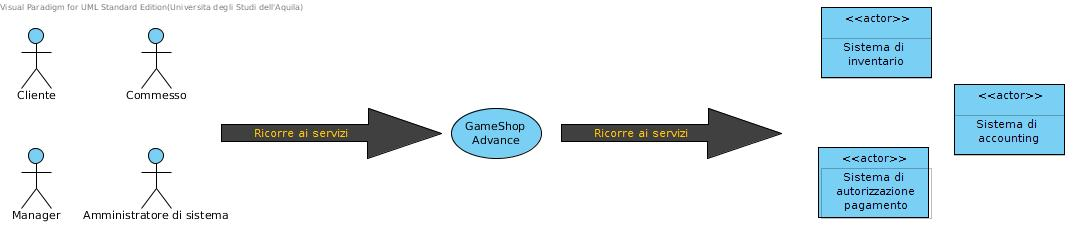
\includegraphics[width=.9\textwidth]{contesto-sistema.png}
 \caption{diagramma di contesto del sistema}
 \label{fig:syscontext}
\end{figure}

  \subsection*{Riepilogo dei vantaggi}
  \begin{tabular}{|p{.5\textwidth}|p{.5\textwidth}|}
   \hline
   \textbf{Caratteristica di supporto} & \textbf{Vantaggi per le parti interessate}\\
   \hline
   In quanto a funzionalità: il sistema fornirà tutti i normali servizi richiesti da un negozio di videogiochi, tra cui la gestione delle vendite, le autorizzazioni al pagamento, la gestione dei resi, \dots &
   Servizi rapidi e automatizzati\\
   \hline
   Regole di business inseribili all'interno degli
scenari durante l'elaborazione delle vendite e
degli scambi di prodotti. &
Flessibilità della logica applicativa,
personalizzazione del business.\\
\hline
Supporto completo alla ricerca e indicizzazione
dei prodotti in catalogo provenienti sia dai
fornitori che dai clienti, sia dal negozio che da
remoto.&
Informazioni aggiornate sui prodotti, semplicità
nel reperirle, maggior organizzazione dei flussi
di prodotti e semplificazione dell'interazione con
i clienti.\\
\hline
\dots & \dots\\
\hline
  \end{tabular}

  \section*{Riepilogo delle caratteristiche del sistema}
  \begin{itemize}
    \item Acquisizione delle vendite
    \item Autorizzazione dei pagamenti
    \item Gestione delle prenotazioni
    \item Ritiro dell'usato
    \item Definizione ed esecuzione di regole di business personalizzate
    \item Indicizzazione dei prodotti e ricerca informatizzata fruibile dai clienti, anche da casa
    \item Gestione dell'inventario
  \end{itemize}

  \section*{Altri requisiti e vincoli}
  Vedere le specifiche supplementari e il documento dei casi d'uso.
\end{document}          
